\begin{figure}
  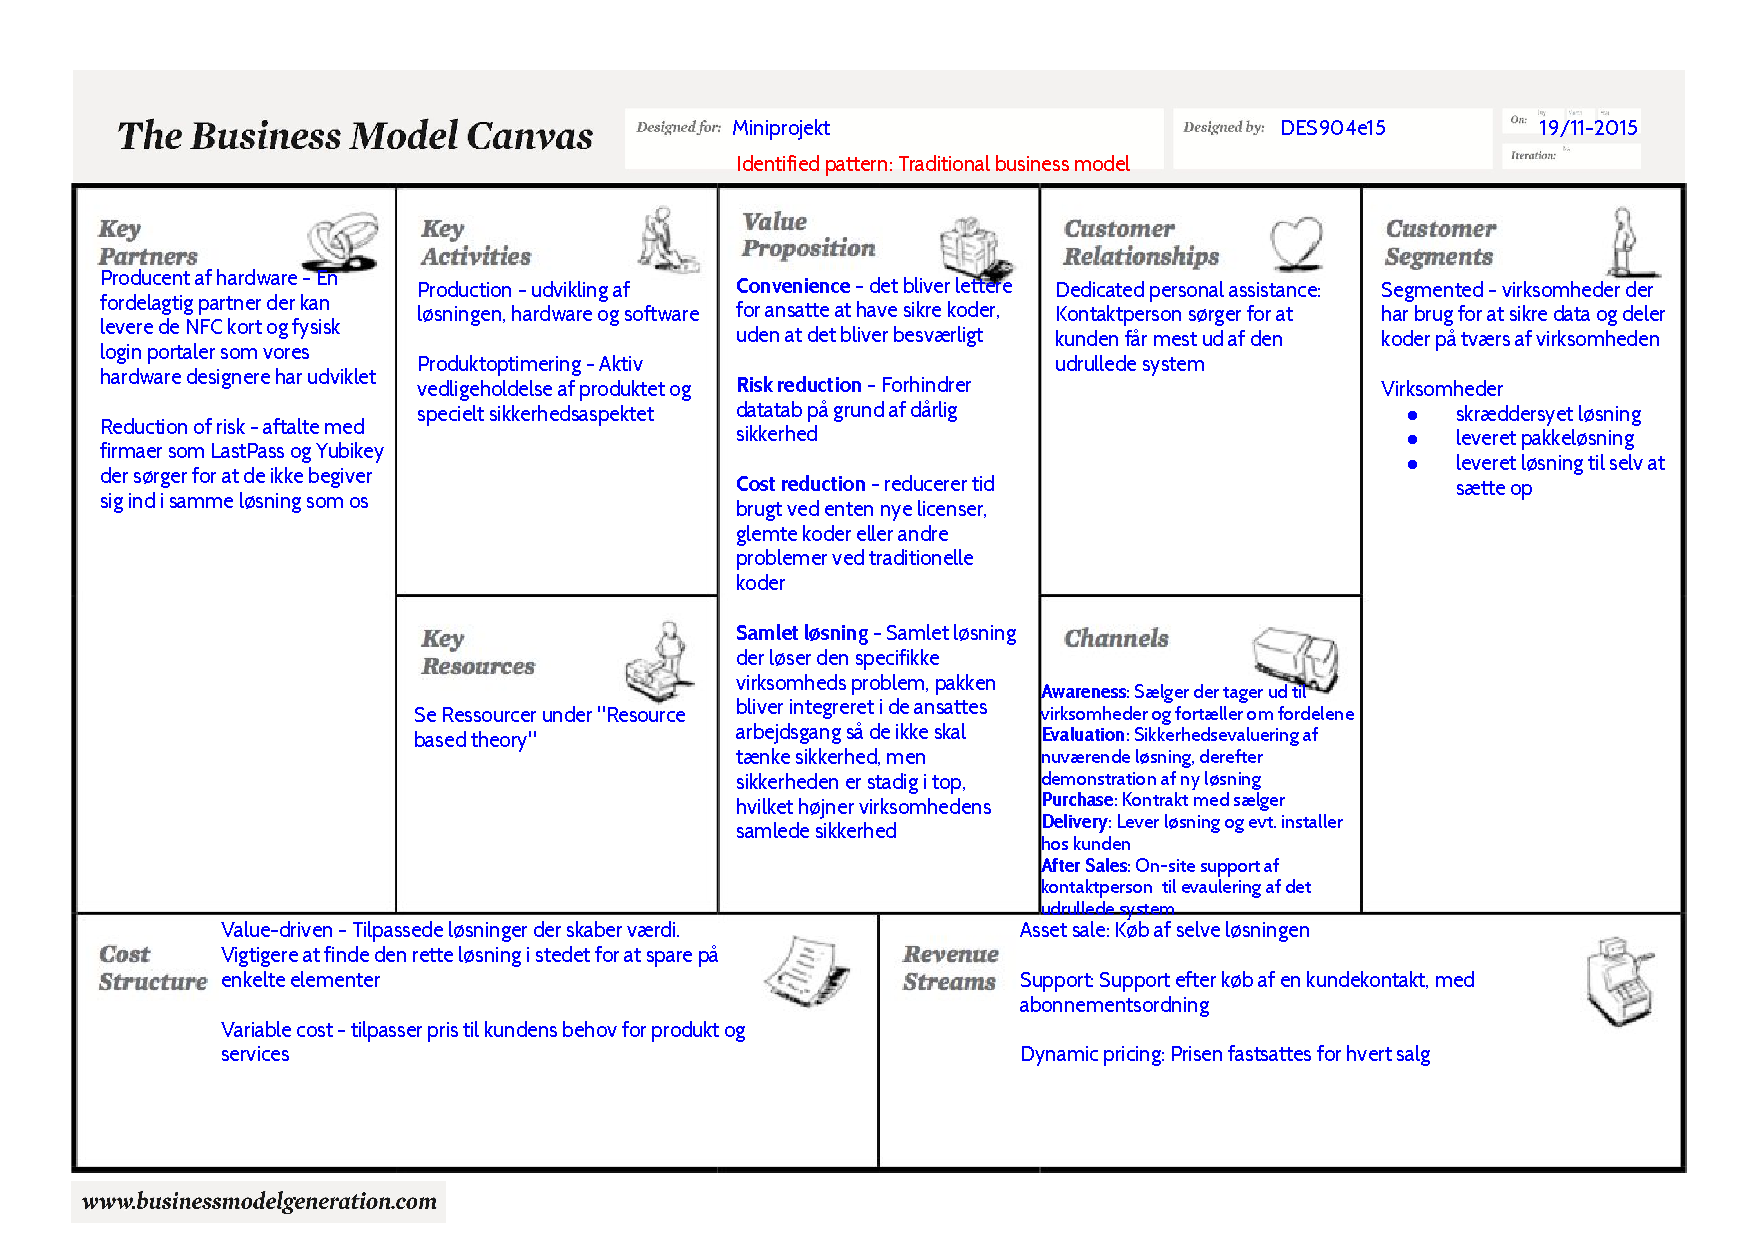
\includegraphics[angle=90, height=0.95\textheight]{graphics/BM.pdf}
  \caption{Business Model Canvas.}
  \label{bm}
\end{figure}

Nu hvor idéen er afklaret og vi har afklaret hvordan vi vil skabe værdi kan vi begynde at designe en business model.
Vi har brugt Business Model Canvas (BMC) fra \citet{osterwalder2009business} til at komme frem til vores business model.
BMC kan bruges til at beskrive, designe, diskutere, udfordre, forbedre og udvikle en BM.
Det er derfor et effektivt værktøj når man er et team med mange forskellige idéer, da det giver et grundlag for bearbejdningen af disse.


BMC består af ni elementer som er med til at sikre at man inkluderer alle væsentlige aspekter af en BM.
Det betyder at man har en liste/skema der kan gennemgås når man ønsker at definere eller bedre en BM.
De ni elementer er: \textit{Customer Segments, Value Propositions, Channels, Customer Relationships, Revenue Streams, Key Resources, Key Activities, Key Partnerships, Cost Structure}.
Vores første BM kan ses på \cref{bm} på side \pageref{bm}.
	